\documentclass[12pt, letterpaper]{article}

\usepackage[margin = 1in]{geometry}
\usepackage{fancyhdr}
\usepackage[english]{babel}
\usepackage[utf8]{inputenc}
\usepackage[doublespacing]{setspace}
\usepackage{graphicx}
\usepackage{pdfpages}
\usepackage{algpseudocode}
\usepackage[toc,page]{appendix}

\usepackage{listings}
\lstset{
basicstyle=\small\ttfamily,
columns=flexible,
breaklines=true
}

\usepackage{caption}
\usepackage{subcaption}
 
\pagestyle{fancy}

\title{Genetic Programming Portfolio }
\vspace{3cm}
\author{James Earle, je11zi@brocku.ca}

\date{Winter 2016}
 
\begin{document}
\begin{titlepage}
\begin{center}
{\LARGE {\bf Genetic Programming Portfolio}}
\\[3cm]
{\large{ \bf \textit{James Earle}}}
{\large \\ Supervised by Dr. Brian Ross}
\\[3cm]
{\large Submitted in partial fulfillment\\ of the requirements for COSC 4F90}
\\[3cm]
{\large Department of Computer Science\\Brock University\\
St. Catharines, Ontario}
\\[5.5cm]
\copyright \textit{ James Earle, $ 2016 $}
\end{center}
\end{titlepage}

\section*{Abstract}

% Here are comments
% 

\textrm{ \indent Genetic Programming (GP) makes use of evolutionary computation to iteratively approximate solutions to a defined problem. When applied to symbolic regression, GP focuses on using a defined language of mathematical functions to derive an equation that closely fits a given target function. In this research, GP with symbolic regression is used as a tool to forecast financial data, namely the Dow Jones Industrial Average (DJIA). Language variations discussed include a simple mathematical language, as well as two more advanced languages that are based in statistical operators and relevant DJIA price data from the past. }

\textrm{ \indent Ensemble learning as it applies to financial forecasting is used to merge multiple predictive models to achieve a stronger, well rounded result. We use ensemble learning in conjunction with an outlier detection system that makes use of a simple $2\sigma$ rule to dramatically improve results and avoid skewed predictions in testing periods. Additional experiments are done beyond language variations that analyse alternate ratios of training data to testing data size. }

\textrm{ \indent A clear improvement in performance is shown when using a training data to testing data ratio of 90-10. This ratio, along with the most advanced finance based language result in the strongest ensemble found. Issues regarding additional functions $avg$, $min$, and $max$ are discussed and considered for long-term forecasting, while their absence was found to be beneficial for short-term analysis. }

\newpage

\tableofcontents

\newpage

\listoffigures

\newpage

\listoftables

\newpage 

\section{Introduction}

\textrm{ \indent The use of artificial intelligence to forecast stock prices is a widely studied field with many major contributions from a variety of perspectives. Much research has applied genetic programming (GP) to this domain, and many varying methodologies have been studied. This provides contrasting results in the literature. In general, GP approaches appear to yield improved results over traditional investment strategies such as the common buy and hold, or day trading. }

\textrm{ \indent GP as it applies to financial forecasting is hindered by the fact that it is common for researchers in this field to not disclose information regarding GP systems or language definitions due to personal benefit from their findings, or corporate investments backing their studies. Due to the large number of factors at play when studying GP, particularly in financial applications, it is very important to consider exactly how parameter decisions will affect the results. Important parameters in the financial field include timing and outcome of quarterly reports, analysis of industry average indicators, changes relative to similar markets, and volume of trade. Important parameters in GP include the GP language, population size, number of iterations, mutation and crossover rates, mutation and crossover techniques, fitness algorithms, and the given language. }

\textrm{ \indent As GP is a probabilistic system, a single run cannot be considered statistically significant in its approximations of a given function. Instead, a stacking, or ``Ensemble Learning'' method will be used as a way to aggregate multiple predictions of the future. This will be used to provide a range of predictions of future welfare, including minimum, maximum, and average approximations across a number of individuals. A programmatic approach to the detection of outliers in ensemble methods will be discussed, as well as a comparison of parameters and language design. }

\textrm{ \indent This research aims to consider GP as a technique for financial forecasting while attempting to address certain gaps in the field. The goal is not to actualize a trading strategy and earn a positive return on investment, rather it is to forecast stock prices with accuracy and robustness in uncertain economic conditions. Additionally, new statistical methods that may prove beneficial in using GP as a tool for price forecasting will be explored. }

\textrm{ \indent The field of genetic programming as it pertains to financial forecasting is rich with ideas of how to create a profitable system that may accurately predict stock prices to some degree. It is hoped that some of the more promising ideas, discussed throughout this paper, will be implemented in the Genetic Programming Portfolio (GPP) system. Different methodologies for both GP and the economic analysis of the problem will be discussed in an attempt to further knowledge of the specific problem of symbolic regression with financial applications. }

\textrm{ \indent In Chapter 2, some background information is given for GP, ensemble learning, and financial forecasting techniques commonly used in econometrics. Chapter 3 will discuss related literature and methodologies used in similar applications of GP, as well as address gaps in the field. A description of the system design in Chapter 4. Here, the program and data processing techniques are explained. Chapter 5 contains the experiments for this research. A detailed discussion on performance benefits based on user requirements and conclusions is then discussed in Chapter 6. }



% add a paragraph sketching the organization of the rest of the thesis

\newpage 
%\addcontentsline{toc}{section}{Background}
\section{Background}

\subsection{Genetic Programming}

\subsubsection{Overview}
\textrm{ \indent Inspired by nature, GP takes an evolutionary perspective on machine intelligence \cite{fieldguide} \cite{koza1992}. It is a variation on genetic algorithms, that is inspired by Darwin's theory of evolution.. In this scenario, small deviations from normality can yield significant improvements in a population of a particular species over a long enough time. These differences allow a species adapt to new environments and challenges, and as it applies to computer programming, approximate a solution to a given problem without an exhaustive search of all potential solutions. Problem solutions are represented by means of a defined programming language. }

\textrm{ \indent Similar to general genetic algorithms, wherein solutions are chromosomes, a language defines functions and terminals as attributes of an individual that are combined and altered throughout the course of evolution to eventually lead towards some ideal solution based on a measure of strength. This measure of strength is referred to as fitness, and is denoted by some heuristic function $f(x)$. There is no best general heuristic function, as a heuristic must be problem specific. For example, in the case of path finding GP systems, the heuristic could be represented as absolute distance to a goal. The general algorithm for GP is shown in detail in table \ref{algorithm1}.}

\begin{table}[!htb]
\centering
\caption{GP Algorithm Pseudo Code}
\label{algorithm1}
\begin{singlespace}
\begin{algorithmic}
\State $pop \gets randomPopulation(popSize);$
\For {$gen \gets 0, maxGen$}
    \State $evaluateFitness(pop);$
    \State $parents \gets selectBasedOnFitness(pop);$
    \State $children \gets applyCrossover(parents);$
    \State $applyMutation(children);$
    \State $gen \gets gen + 1;$
\EndFor 
\\
\Return $bestIndividual;$
\end{algorithmic}
\end{singlespace}
\end{table}

\subsubsection{Parameters}
\textrm{ \indent System parameters influence the ability of a GP system. Crossover and mutation are two standard operations among GP that behave analogously to their real world counter parts. Between generations, candidate solutions will breed, sharing features of their chromosomes with one another and creating a new individual from the combined result. This is referred to as crossover. Similarly, mutation modifies the chromosome of an individual. This function is asexual, in that it does not require two parent candidates to be performed. }

\textrm{ \indent In GP, selection algorithms are commonly put in place to determine which individuals from the population will breed based on their fitness. The most common is tournament selection, where a number of individuals are chosen at random and the most fit individual will be chosen to perform some action. In the case of crossover, two tournament selections will take place to select each parent. }

\textrm{ \indent Elitism is another common feature of genetic algorithms. The best individuals at each iteration are never altered, and simply move into the next generation unchanged. This allows GP to retain the most fit individuals. }

\subsubsection{Defining a Language}
\textrm{ \indent GP systems adhere to a language defined by a function set and terminal set. Functions are $n$-ary operations defined as taking parameters of a certain type. Terminals are parameters to a function, or constant value. For example, the $+$ function is a binary function, so can be written as $ +(a, b) $. In this case, $a$ and $b$ could themselves be functions or terminals. A terminal could be an initially randomly generated value, referred to as ephemeral random constants (ERC). This exists throughout an entire GP run without variation. Terminals can also be represented as a stream of values. In this case, variables can be time dependent. This means that all functions and terminals that exist as a time-series must be sampled within the same time period by the GP system each generation. In doing this, significant improvements can be made to a language as GP is now considering data across time.}

\subsubsection{Data Representation}
\textrm{ \indent Functions can a tree-based representation. Any given individual is initialized as a random combination of these functions and terminals, with each existing as a node in the tree. Over time, they are ranked for their performance against a specific problem and set of training data using some heuristic function. Individuals in the population are then bred using crossover and mutation to share genetic attributes and create entirely new solutions probabilistically. Given enough generations, strong attributes will appear through evolution and can represent significant features of the problem itself. Crossover and mutations take place at nodes of the same type in tree based symbolic regression, ensuring syntactic correctness of candidate solutions after a transformation. }

\subsubsection{Tree Generation}
\textrm{ \indent Two tree generation methods are used, namely \textit{full} and \textit{grow} \cite{fieldguide}. In the \textit{full} methodology, trees generated always have all leaves at the same depth. Functions are chosen from the function set until a user specified depth is reached, after which only terminals can be chosen. The \textit{grow} method is similar to \textit{full} in that a user specified depth is required. Functions and terminals are chosen at random until the tree reaches the specified depth, but in the \textit{grow} technique it is possible to choose terminals before the depth limit is reached. This allows for the creation of trees varying in size and structure. }

\textrm{ \indent Koza proposed a technique called \textit{ramped half-and-half}. Ramping allows trees to be generated having different sizes (depth). This method creates half of the initial population using \textit{full} and half using the \textit{grow}. This allows trees that can be very large and well balanced, as well as a variety that are very unbalanced. This diversity of a population, akin to nature itself, promotes strength in evolution across generations. }

\subsubsection{Symbolic Regression}
\textrm{\indent It is common that GP systems applied to stock selection will either use symbolic regression or rule-based GP to create price forecasting models. Symbolic regression is used to generate mathematical expressions that fit a given function. It can be used to create a function that will accurately predict previously unknown inputs by learning important features of the target function. Common econometric techniques are able to more closely be compared to a given mathematical function as a result of a GP run to quantify levels of efficiency and errors. The general approach in either case, however, is similar. A system must be trained on selected data before being applied to unknown data and verified. It is desirable that the training period provides accurate example behaviour of how the economy generally behaves, so that the returned function can remain robust when given unknown data. It is for this reason that the choice of training data is very important, as it must be representative of typical economic behaviour. Many econometric techniques that approach price forecasting use symbolic regression, and many of these techniques also use mean squared errors as an indicator of strength in a specified model. For symbolic regression problems in GP then, the heuristic function will be defined as the squared residuals between the target data and the models specification. }


\subsection{Ensemble Learning}

% currently have 3 papers on ensemble learning. Discuss generally as a concept before bringing GP into it. 
\textrm{\indent A common approach in machine learning is to allow for multiple varying models to make a decision collectively \cite{ensemble-wiki}. This provides safer approaches to predictive problems by allowing multiple systems to express opinions that can then be aggregated by some fusion technique into an overall estimate. Fusion techniques of individuals vary based on the problem domain. They regularly involve weighing the decisions of the multiple individual predictive models in such a way that it can be assured there is strength in the aggregate ensemble. }

\textrm{ \indent Outliers in ensemble learning pose a serious problem. When fusing individual models into an ensemble, outliers have the ability to substantially skew the overall result while remaining invisible unless a detection system is put in place. Similar to fusion techniques, classification of outliers in an ensemble learning approach is a domain specific problem. As it applies to GP and symbolic regression, ensemble learning is an excellent tool to be applied for financial forecasting. Fusion techniques can be simply the average or median functions across a specific set of models. In this case, outlier detection requires the ability to classify data points that lay a significant distance beyond the ensemble average.  }

\subsection{Financial Forecasting}

\textrm{ \indent Many common econometric forecasting techniques exist, such as Ordinary Least Squares (OLS) regression testing, the Classical Linear Regression Model (CLRM), and non-linear models, such as Maximum Likelihood Estimation (MLE) \cite{econometrics}. Each has their drawbacks. OLS and the CLRM rely most prominently on the assumption of linearity in the estimated data and a fixed sample size. Additionally, OLS relies on non-heteroskedastic errors. This means that as the model predicts further and further into the future, the errors are not increasing in size. MLE is a more diverse estimation technique that allows for non-linear models. Additionally, MLE generally works in $log$ models and as a result is able to deal with non-linear models in a linear fashion. This provides unbiased and efficient estimates of a given regression model. }

\textrm{ \indent The closest similarity that can be drawn between conventional financial forecasting and GP with symbolic regression is the traditional OLS model. In OLS regression testing, a model is specified with unknown coefficients. These coefficients are then estimated to minimize the mean squared error surrounding the target data. This is analogous to GP and symbolic regression, except that symbolic regression does not rely on a strictly specified model of any particular form. It is able to dynamically create a model as evolution takes place. This has benefits in that it is not forcing the data into a certain perspective under a given model, but requires the additional work of elongated exploration of search space to perform this regression. }

\textrm{ \indent To aid the GP system in forecasting financial data, it is wise to add financial and statistical language elements to the function and terminal sets. This follows in the logic any person could take in trying to forecast the stock market independently: more information means more accurate forecasting. Rather than attempt to do so using only symbolic math estimates, one would also incorporate historical price data and relevant statistical information in their estimates. This ensures that GP's information set at as knowledgeable as possible. }

\newpage 

\section{Literature Review}

\subsection{Financial Forecasting}

\textrm{ \indent Symbolic regression problems are sensitive to the role that a large training dataset will play on a system, as well as how known features of a dataset will manipulate results. For their research, Kim \textit{et al.} \cite{overfitting} chose the S\&P 500 index from January 1990 to December 2006. This period of 16 years provides a surge of growth in multiple markets, as the S\&P 500 is known to be a strong reflection of real economic welfare. The choice to end in 2006 is likely made in order to avoid modeling the undesirable economic state of 2007-2009. It is argued that severely abnormal economic behaviour is not ideal for building a robust system. Recessions are seen as uninformative in that they model unusual behaviour, which in practice tends to skew econometric models. }

\textrm{ \indent Having a model overfit training data is a common occurrence among symbolic regression problems, and machine learning in general. This is done by too closely fitting a particular data set that will map that exact behaviour onto the testing data. This ignores potentially informative attributes in the data, and instead memorizes a pattern seen in training. Kim \textit{et al.} \cite{overfitting} have approached this problem by creating an objective function, dividing the generation of a system into three steps. First is the training step, where the selected period of training data is divided into two subsections. Here, each half of the data is given to two separate runs of the GP system, and are compared and merged upon completion. An interesting variation of this part of the process would be running two independent test GP systems on different data sets, perhaps one containing a recession and another with more usual economic behaviour. This could possibly point towards some merged behaviour that, on average, can perform well even under poorer circumstances. After the runs have complete, the best candidates in each GP are then run again on the remaining half of the data, along with new random candidates. Finally, in the validation step, the best models performance are evaluated and analysed on entirely new data. }

\textrm{ \indent It is uncommon for financial researchers to reveal specifics regarding their GP implementation, or even more so their specific fitness functions. Kim \textit{et al.} \cite{overfitting} have provided this detailed and problem specific guide to structure the creation of a strong GP that is resilient to overfitting of data. The key to the robustness against overfitting in their experience is that the chosen tree depth is constrained to substantially beyond what is considered typical. Many other researchers such as John Koza \cite{treesize} have spoken on this topic, using values larger than Kim has chosen. This is an interesting choice, as a large tree can allow a GP to be ``lazy'' and select less promising or factually representative trees that just yield a high fitness, while small trees can force more representative functions that do not allow too much detail, ignoring noise in data. Conversely, small tree sizes can restrict possibly good solutions, while large tree sizes can leave large portions of the tree completely useless, a common occurrence normally referred to as bloat. An example of this is if the given language contains a conditional function, but GP has used it in such a way that the condition test is always true or always false. Anything in one of its branches is dead weight, but still renders a marginally higher fitness acting as a safety net and will be kept. }

\textrm{ \indent Korns \cite{korns} focuses on constrained symbolic regression problems for financial applications and aims to challenge commonly held beliefs that are considered the norm in academia, as well as aggregate multiple ideas he believes to be more accurate than others. The particular focus involves symbolic regression on a large scale, since within economic applications it can be expected that there will be many large datasets. GP behaviour depends significantly on the chosen granularity and length of training and verification data. In data-rich environments Korns discusses the different possible sampling methodologies that can be taken in opposition to sampling an entire dataset. Korns chooses to use 1250 days of data for 800 common stocks as training data. This resulted in a total of 1,000,000 data entries. A large factor regarding his decision is the time it takes to process the information and retrain his system regularly, as the expected time to finish training periods is 50 hours. In doing this, his goal is to analyse how well the standard population size, crossover rate, etc. will work in large scale problems, and consider alternate values for these parameters. }

\textrm{ \indent Korns' training process described is simpler than what is discussed previously by Kim \textit{et al.} \cite{overfitting}, in that the process is less rigorous, given the quantity of data. Rather, the system is run on 9 test case formulas ranging in difficulty, with the inclusion of functions that add random noise. Economic data is already very noisy, and it is hard to pinpoint whether or not the data may have underlying factors attributing to its behavior that may not have been accounted for. The intentional addition of noise to data is not standard practice among researchers who have focused on econometric applications. }

\textrm{ \indent Korns \cite{korns} uses a hybrid grammar and tree-based GP. Experiments consider a variety of test case formulas, ranging from simple linear equations to complex ellipses, as well as mixed formulas that use Boolean operators. This shows some promising results on the simpler functions, yet it thought possible that the addition of noise made it difficult to come up with such results in more complex scenarios. To account for the magnitude of the problem, he also uses lengthy runs, with a large number of generations.  }

\textrm{ \indent Korns \cite{korns} mentions the simpler data points such as open, high, low, close, volume, earnings per share (EPS), and analyst rating as being valuable in price forecasting. Despite the simplicity of these indicators, Korns argues that they are essential, as they act as a baseline of data describing market behaviour. This contrasts the opinions of Kim's \cite{overfitting} work in discussing the overfitting of GP systems, mentioned previously. The nature of simplicity in these indicators is a double edged sword, as they are also the most widely available. Even the simplest stock portfolio application will track this information. Although specific relationships are not shown, to maintain trade secrets, descriptions are associated with each variable in Kim's \cite{overfitting} description of their GP system. The chosen indicators are noticeably more sophisticated, using variables such as dividend yield, profit and growth margins, and net debt ratios. Additionally, analyst long-term estimates have been chosen despite a discussed apparent variability in these ratings. }

\textrm{ \indent Becker \textit{et al.} \cite{stockselectinnovate} take a stronger economics perspective in their work than in many of the previously mentioned papers. Despite the problem of symbolic regression being purely mathematical, it is important to remember that any additional, problem specific, information that can guide a GP to a more adequate and robust solution is ideal. Becker chooses to analyse the S\&P 500 index, as it is an aggregate of information on the overall economic well being at any time for 500 large companies traded publicly on the NASDAQ. Attributes associated with an aggregate index in this case are argued as being representative of generic economic welfare, and in this case bring substantial value and robustness to a symbolic regression model. } 

\textrm{\indent Kaboudan \cite{kaboudan} explores the topic of actualizing a GP system to make real trades. Very strong econometric methods are used to analyse the performance of the given GP. It is hypothesized that a single day trading strategy (SDTS) is likely the most profitable. However, specifics regarding his language or parameters were not mentioned. This study finds that by analyzing previous data up to the present day it is possible to make accurate predictions regarding tomorrow's performance. Any efforts exceeding a day seemed to yield next to no return, or at the very least no statistically significant advantage of regular trading strategies, such as buy and hold.}

\textrm{ \indent Kaboudan \cite{kaboudan} notes that this method comes with a set of drawbacks. If the forecasted increase is not enough to justify the risk, as well as the cost of performing the trade, then of course a trade will not be made. He also adds that if the actual prices fall below the forecasted low, or above the forecasted high, then again a trade will not be made. It is understood that this is a safety precaution because otherwise the forecasted profit cannot be relied upon. However, it is not necessarily true that an opening price lower than the forecasted opening price is necessarily bad. It can be a sign of a failing stock, but also a sign of an undervalued stock. The distinction between the two, while difficult to make, can be very important. Kaboudan \cite{kaboudan} presents all of the logistics regarding actualizing a GP that forecasts stock prices well, but does not provide information regarding implementation of the system itself. Despite this, econometric analysis in this work will provide useful techniques towards evaluating performance of a GP. }

\textrm{ \indent Similar to the work of Kaboudan \cite{kaboudan}, Mallick \cite{mallick} aims to implement a stock trading system based purely on trading rules created in a GP based system. Trading rules create an environment of binary yes/no questions that lead to a buy or sell decision on the chosen stock. He does not include details on the chosen language, but does provide details regarding GP parameters. The system parameters fall slightly lower than what is seen in alternate literature. Similar to Kaboudan \cite{kaboudan}, comparisons are drawn from the implemented trading strategy to the common buy and hold technique, as well as the MACD (Moving Average Conversion/Diversion) technical indicator. This indicator is a highly praised accurate forecasting method of the general direction a stock is likely to drift towards. }

\textrm{ \indent Contrary to many of the previous works, an alternate perspective of approaching this problem is focus on the model itself. The above use a time-period based model. Some used daily data, while others used longer time periods in an attempt to aggregate general behaviour and remove granularity from the problem. Gypteau \cite{gypteau} argues that using physical time intervals is a poor structure for the problem at hand. He instead proposes event-driven models. Models that are event-driven do not rely on sequential data. Instead, they focus on significant occurrences in the media or stock market that can be expected to invoke change. A large amount of analysis is required in order to automate the process of deciding what is and is not a significant social event that will impact a particular market. This may seem easy in the case of analyzing quarterly reports, but an important aspect to the problem is general market mood. Bollen \cite{twitter} argues that Twitter is able to accurately predict the stock market based on overall moood, as human emotions profoundly drive our decision making process. In his specific work, he forecasts the mood of Twitter in an aggregate manner daily and compares it to the public's response to the presidential election, and finds very positive results. } 

\textrm{ \indent Autocorrelation and business cycles are two important concepts that should be recognized in financial forecasting. In an economics-oriented GP survey, Navet \cite{navet} discusses the statistics behind use a time lag and analyses the entropy of given stocks to find out if low entropy stocks are more profitable than those with higher entropy. There is little mention of the GP system used, besides a brief introduction to GP as a whole, but the use of time lagged data comparisons is interesting as dependence of today's market values on yesterday's is a highly debated topic among economists. }

\subsection{Ensemble Learning}

\textrm{ \indent Ensemble learning has the potential to greatly improve machine learning experiments that are probabilistic in nature such as GP. Ensemble learning can be implemented by running the system multiple times concurrently, and aggregating the results. Veeramachaneni \textit{et al.} \cite{ensemble1} have chosen to analyse GP and symbolic regression at scale in a dynamic data-driven system, while simultaneously altering parameters for different runs that are included in the ensemble. This allows a diverse set of models that will have noticeably different outcomes, and thus a strong prediction across the ensemble after fusion has taken place. }

\textrm{\indent There exist many ways to fuse individual models into an ensemble to form a single forecast \cite{ensemble1}. Some ensemble learning techniques in GP include average ensemble prediction (AVE), median average model(MAD), and adaptive regression mixing (ARM) \cite{ensemble1}. AVE and MAD are similar in nature, finding the average or the median among the discrete set of models respectively. The ARM ensemble approach is more complex, assigning weights to each model to represent how important its prediction should be in the aggregated result. These weights are generated as a result of confidence in each specific model. Through the work of Veeramachaneni \textit{et al.} \cite{ensemble1} it is found that traditionally simple techniques of fusion, such as AVE and MAD do not yield strong results comparatively. }

\textrm{\indent It is not uncommon in ensemble learning to use entirely different machine learning techniques to provide the highest level of diversity of models for a single problem. Symbolic regression is a particularly flexible problem, and as such is open to many such techniques. Veeramachaneni \textit{et al.} \cite{ensemble2} use many cloud-based platforms for comparison to their own system, which also makes use of feed forward neural networks, multi-objective genetic programming, and optimized multi-objective genetic programming. These systems are run in parallel, and Veeramachaneni \textit{et al.} goes on to discuss different ensemble fusion techniques as well as best approaches for concurrent division of datasets. It is found that feed-forward neural networks provide the strongest predictions in the ensemble, and when used in a cloud-based application provide extreme efficiency as GP alone requires significantly more time to complete the same operations. The use of multiple, completely different machine learning techniques in an ensemble is one that certainly is shown to yield positive results due to the differing natures of each technique. }

\begin{figure}[!htbp]
\begin{center}
\includegraphics[width=\textwidth]{eureqa}
\end{center}
\caption{Eureqa Revenue Projection.}
\label{eureqa}
\end{figure}

\textrm{ \indent An industry application of GP using symbolic regression in financial forecasting is given by Nutonian Inc. \cite{eureqa}. In Figure \ref{eureqa} a price forecast is shown. A cone shape is seen forming around the projection. This is what has been described earlier by heteroskedasticity. Errors are increasing as time goes on in the forecasted data. Eureqa focuses on hedge fund operations to provide projections to customers for their business growth. The specifics of the system are not given, beyond that GP is used with symbolic regression. This service provides an interesting perspective on the use of GP in an applied approach to financial forecasting. }

\newpage 

\section{System Design}

\subsection{ECJ \& GP Language}

\textrm{\indent Developed at George Mason University's Evolutionary Computation Lab, ECJ is a diverse library providing access to classes and interfaces that promote efficient programming \cite{ecj}. All system parameters are determined at runtime by a user-defined file, which can be read from and altered without the need to rebuild the system. To create an instance of a GP system using ECJ, the user need only provide an implementation file, data type file, and classes representing function and terminal sets. }

\textrm{ All evolutionary operations, such as crossover, mutation, elitism, and handling generations are handled by ECJ. The methodologies follow those discussed by John R. Koza \cite{koza1992} by default, but the user is free to override this behaviour, providing a flexible framework. This allows the user to focus entirely on the problem definition and higher level analysis, such as the GP language. }

%\textrm{ A GP language definition is generally considered stronger when it uses as much problem-specific data as necessary. In the case of symbolic regression, it is required to have a number of mathematical operators however when used for financial forecasting it is also extremely beneficial to provide financial data and statistical analysis functions as well. The ability to include these functions in the system is supported in part by ECJ, allowing for external data access at runtime. All data to be used at runtime is read from a file and stored in the implementation file. }

\subsection{Fitness Evaluation \& Ensemble}

\textrm{ \indent The sum of squared errors is used to evaluate fitness of GP models. Each individual model will have it's own fitness score that is evaluated after execution. A Python script will process output from each run and calculate the difference between the target data and the model projection into the future. This allows the system to sort runs by fitness. }

\textrm{ \indent When aggregating GP results and building the ensemble, the system will always check if any data point exceeds $\pm2$ standard deviations, or $2\sigma$, from the average. All data points that violate this rule are removed before the ensemble average or median at this time interval is recalculated. }

\textrm{ \indent Ensembles are created through use of average and median fusion techniques. The average fusion technique will average 20 models at each data point to create a new curve. The median fusion technique will behave similarly, only taking the median of the 20 models at each data point instead. As the Python script is executing an individual runs output is recorded and saved. Afterwards the execution continues to create a new model that is the average, or median, of the 20 individual runs. This is where the $2\sigma$ outlier detection rule is put in place. Should any individual data point exceed $2\sigma$ above or below the ensemble value, it is removed and the value at this data point is recalculated. After the ensemble has been aggregated, a score is calculated by iterating the target data and comparing using the sum of squared errors.}

\subsection{Data Processing}

\textrm{ \indent To aid in processing important data of system executions, a Python interface has been included in the project implementation. This includes a variety of Python scripts that serve varying purposes, such as graphing data or aggregating it into a format that is easier to manipulate. The choice of Python as a processing language was based in ease of use, as there exists many statistical analysis and graphing libraries. Additionally, Python is easily capable of being executed from the Java runtime in which ECJ and the bulk of the GP system is implemented. }

\textrm{ \indent From the main ECJ execution file, a proxy Java class is called that is responsible for executing the Python scripts and handling their output. At this point, a variety of text files are created that include data on the best of run individuals for every execution, as well as other important statistics like standardized and adjusted fitness. This allows a high level of automation for repetitive analysis tasks as well as aids in formatting for Microsoft Excel spreadsheets. }

\begin{figure}[!htbp]
\begin{center}
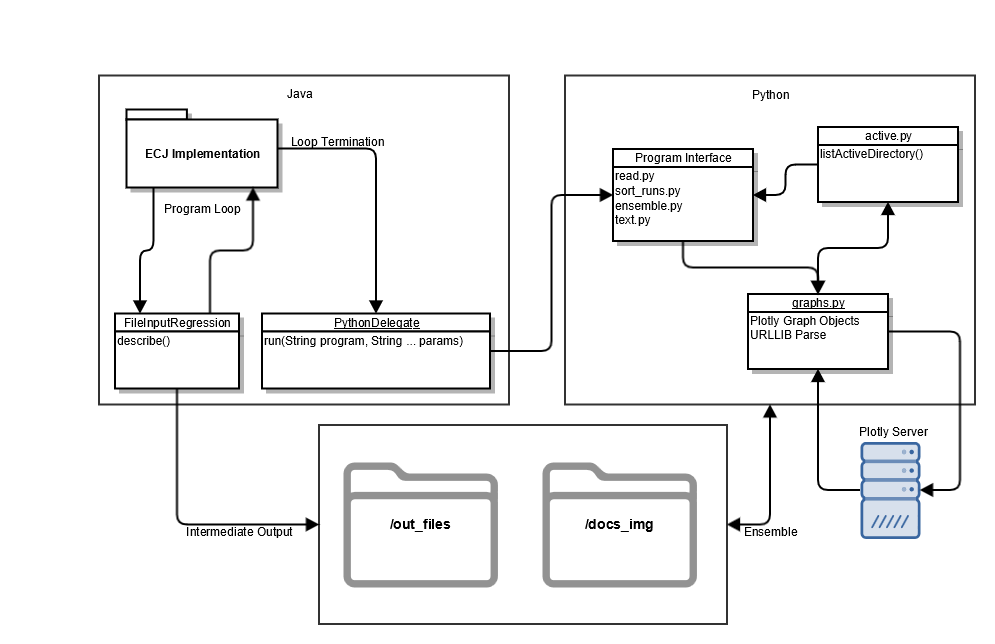
\includegraphics[width=20cm,angle=-90]{system_design.png}
\end{center}
\caption{Design of the GPP System.}
\label{fig:system}
\end{figure}

\textrm{ \indent Figure \ref{fig:system} shows details of the system design. The flow of data as it is created and processed by Java and further processed by the Python interface is described. Information on the fitness of every generation in every run is stored as intermediate output periodically as raw text files. The Python interface then reads this intermediate output, aggregating it to provide an average look across runs, so that no individual, coincidentally strong run skews perceptions regarding system performance. Additionally, once at the end of each run Java will output extra details regarding the best of run individual into a separate directory. Here, Python sorts them and applies ensemble learning methodologies, such as outlier detection in the ensemble, as well as simple average, median, minimum, and maximum data. }

%%%%%%%%%%%%%%%%%%%%%%%%%%%%%%%%%%%%%%%%%%%%%%%%%%%%%%%%%%%%%%%%%%%%%%%%%%%%%%%%%%%%%%%%%%%%%%%%%%%%%
%%%%%%%%%%%%%%%%%%%%%%%%%%%%%%%%%%%%%%%%%%%%%%%%%%%%%%%%%%%%%%%%%%%%%%%%%%%%%%%%%%%%%%%%%%%%%%%%%%%%%
% Follow: Setup, Results, Discussion
%
% March 28, 2016 - Notes from meeting with Ross
%
% Each experiment should follow this structure
% 
% SETUP - Language, data, previous exp acknowledgements
% RESULTS - Graphs, short descriptions, touch on features of data, "what"
% DISCUSSION - "why"
%
% Below is the generic format for all of section 5
%
% Math
%   no-iflt
%       avg vs. median ensemble
%   with iflt
%   outliers
% Statistics
%   prelim: < 50% spaces
%   95%
%       avg, min, max. Include and discuss pitfalls (or "rules")
%   90%
%   75%
% Finance
%   vol, open, high, low
%       discuss with avg, min, max, again (maybe)
%
%%%%%%%%%%%%%%%%%%%%%%%%%%%%%%%%%%%%%%%%%%%%%%%%%%%%%%%%%%%%%%%%%%%%%%%%%%%%%%%%%%%%%%%%%%%%%%%%%%%%%
%%%%%%%%%%%%%%%%%%%%%%%%%%%%%%%%%%%%%%%%%%%%%%%%%%%%%%%%%%%%%%%%%%%%%%%%%%%%%%%%%%%%%%%%%%%%%%%%%%%%%

\newpage

\section{Experiments}

\textrm{ \indent The following experiments aim to analyse language variants in GP in an attempt to find efficient financial forecasting solutions. The use of a Boolean function is considered in conjunction with a simple math language, after which more functions are added that focus on 5 day time-delayed statistical and finance operators. Results are contrasted with and without newly added functions to observe their effect, as well as compared based on a training data to testing data size ratio. After this, final conclusions are drawn regarding performance of GPP given the proposed language variants as well as the defined use case of price forecasting in the long and short run. }

\subsection{Preliminary Trials \& Data Selection}

\textrm{ \indent Preliminary experiments that focused on parameter decisions found noticeably superior results given the parameters shown in Table \ref{fig:params}. They will be used in the subsequent experiments. Crossover, mutation, elitism, and tournament size follow the typical behaviour described in Section 2.1. The maximum tree depth specified refers to the initial randomly generated population that uses \textit{ramped half-and-half} \cite{fieldguide}. Population size describes the number of candidate solutions initialized and bred throughout each generation.}

\textrm{ \indent Although forecasting very brief, volatile moments in time presents a significant challenge for GP when using symbolic regression, long term trends are where it excels. Different time ranges are considered in the following experiments, in particular the ratio of training data to testing data is explored. Dow Jones data is used between January of 2013 to January of 2016 to provide 3 fiscal years of data to explore. The data provides a wide range of economic behaviour that allows for a diverse GP training set. Additionally, data has been normalized to fall in the range $[0, 1]$ for the purposes of human interpretation as well as simplicity in fitness calculations and defining a numeric range for other variables of significance.}

\begin{table}[!ht]
\centering
 \begin{tabular}{||c|c||}
 \hline
 \textbf{Parameter} & \textbf{Value}  \\ [0.5ex] 
 \hline\hline
 Crossover & 90\% \\ \hline
 Mutation & 10\% \\ \hline
 Elitism & 0 \\ \hline
 Tournament Size & 2 \\ \hline
 Max Tree Depth & 17 \\ \hline
 Pop. Size & 1000 \\ \hline
 Generations & 100 \\ \hline
 Runs & 20 \\ \hline
 \hline
\end{tabular}
\caption{GP Parameters.}
\label{fig:params}
\end{table}

\subsection{Experiment 1: Mathematical Language}

\subsubsection{Setup}
\textrm{\indent In this experiment, the use of simple mathematical operators is explored and contrasted with the use of an additional Boolean function, namely \textit{if less than}, or $IFLT$. This function is defined as $ IF(a<b)\ RETURN\ c\ ELSE\ RETURN\ d$, where $a$, $b$, $c$, and $d$ are parameters to the function. }

\textrm{ \indent The choice of only having an \textit{if less than} function came from the precision required to compare equality for floating point values. The difference in function behaviour is negligible in nearly all circumstances. Additionally, there is no greater-than function because $a<b \Rightarrow b>a$, and so any similar additional Boolean functions would be redundant. }

\begin{table}[h!]
\centering
\begin{tabular}{||c|c||}
\hline
$L$ & $x$, $ERC$, $+$, $-$, $\times$, $\div$, $log$, $cos$, $sin$ \\
\hline
$L_{IF}$ & $L \cup \{ IFLT \} $ \\
\hline
\end{tabular}
\caption{Math Language Definition}
\label{math-lang}
\end{table}

\textrm{ \indent The language variations $L$ and $L_{IF}$ used in the first experiment are defined in Table \ref{math-lang}. Here $x$ represents day number in the data, and $ERC$ represents ephemeral random constants, as floating point values. The ERC value is set at the beginning of each run and is invariant between generations, while $x$ exists in the closed range $[0, n]$, where $n$ is given by the number of data points being sampled. }

\textrm{\indent The training data used in this experiment is the first 90\% of the data, consecutively. GP will perform symbolic regression on this data set. The testing data is then the remaining 10\% of unseen data. After the run has completed, the model will be evaluated on unseen data in the testing range to evaluate performance. The training data set consists of 702 data points, with 78 data points remaining in the testing range. Differing ratios for ranges, such as 80-20 and 70-30 training to testing respectively are considered in the experiments that follow. }

\subsubsection{Results}

\begin{figure}[!htb]
\begin{center}
\includegraphics[width=\textwidth]{exp1/no-iflt/best-avg-training}
\end{center}
\caption{ $L$ Training of Best vs. Average Individuals.}
\label{fig:no-iflt-best-avg-train}
\end{figure}

\textrm{ \indent In Figures \ref{fig:no-iflt-best-avg-train} and \ref{fig:with-iflt-best-avg-train}, the entire individual models are shown for without and with $IFLT$, respectively. Interestingly enough, there is a clear trend of highly volatile cycles in both individuals in Figure \ref{fig:no-iflt-best-avg-train}, but not in Figure \ref{fig:with-iflt-best-avg-train}. This type of behaviour is typical of GP systems that use $cos$ and $sin$ functions. Notice that these cycles persist less in the testing data, with the exclusion of the average individual shown in Figure \ref{fig:no-iflt-best-avg}. }

\begin{figure}[!htb]
\begin{center}
\includegraphics[width=\textwidth]{exp1/with-iflt/best-avg-training}
\end{center}
\caption{ $L_{IF}$ Training of Best vs. Average Individuals.}
\label{fig:with-iflt-best-avg-train}
\end{figure}

\textrm{ \indent Figure \ref{fig:no-iflt-best-avg} shows the target test data plotted against the strongest individual model in the ensemble, as well as an average fitness model under $L$. Figure \ref{fig:with-iflt-best-avg} shows the same with the additional functions in $L_{IF}$. Both show the performance on previously unseen data. It is clear to see that this results in more fit individuals and with the use of $IFLT$ points to an interesting combination of language functions that may lead to improved performance. The GP trees for the best model in the ensemble under $L$ can be seen in Appendix \ref{appendix-a}, and likewise for the best model in the ensemble under $L_{IF}$ in Appendix \ref{appendix-b}. }

\begin{figure}[!htb]
\begin{center}
\includegraphics[width=\textwidth]{exp1/no-iflt/best-avg-compare}
\end{center}
\caption{ $L$ Testing of Best vs. Average Individuals.}
\label{fig:no-iflt-best-avg}
\end{figure}

\textrm{ \indent Both models highlight interesting features in the target data considering the use of a language based only in math functions. Both individuals have relatively smooth curves, but the use of $ILFT$ clearly creates sudden breaks and highly volatile moments in time, including some perfectly vertical jumps. It is also interesting to note that the most fit individual in the entire ensemble without use of $IFLT$ seems to be increasing, relatively linearly. This is not the case with the average individual that has more fluctuations in a cyclic, downward sloping fashion. }

\begin{figure}[!htb]
\begin{center}
\includegraphics[width=\textwidth]{exp1/with-iflt/best-avg-compare}
\end{center}
\caption{ $L_{IF}$ Testing of Best vs. Average Fit Individuals.}
\label{fig:with-iflt-best-avg}
\end{figure}

\textrm{ \indent Consider the performance statistics shown for Figures \ref{fig:no-iflt-best-avg} and \ref{fig:with-iflt-best-avg} in Table \ref{no-iflt-ind-stats}. It is seen that using the $IFLT$ function in the language yields higher fitness in both of the shown individuals. The difference with and without is more prominent for the best individual. This describes the performance of the language in such a way that multiple diverse individual models are generated that may not always agree.}

\begin{table}[!ht]
\centering
\begin{tabular}{||c|c|c||}
\hline
\textbf{Category} & \textbf{Average Fit Ind.} & \textbf{Most Fit Ind.} \\
\hline
 $L$ & 0.251398 & 0.120458 \\
\hline
$L_{IF}$ & 0.232546 & 0.097193 \\
\hline
\end{tabular}
\caption{Average Fit Individual \& Most Fit Individual Performance}
\label{no-iflt-ind-stats}
\end{table}

\begin{figure}[!htb]
\begin{center}
\includegraphics[width=\textwidth]{exp1/no-iflt/ensemble-high-low}
\end{center}
\caption{ $L$ Average Ensemble vs. Median Ensemble.}
\label{fig:no-iflt-avg-med}
\end{figure}

\begin{figure}[!htb]
\begin{center}
\includegraphics[width=\textwidth]{exp1/with-iflt/ensemble-high-low}
\end{center}
\caption{ $L_{IF}$ Average Ensemble vs. Median Ensemble.}
\label{fig:with-iflt-avg-med}
\end{figure}

\textrm{ \indent Figures \ref{fig:no-iflt-avg-med} and \ref{fig:with-iflt-avg-med} shows the ensemble using both average and median approaches to fuse individual models from the ensemble under both $L$ and $L_{IF}$. Additionally, minimum and maximum data points from individual models are kept and plotted to create high-low lines representative of a forecasting range. It can be seen that both average and median ensemble techniques perform relatively the same, with some initial volatility then tapering off as time goes on. This applies to both ensembles, with and without $IFLT$. Automatic outlier detection is put in place to avoid skewed ensembles. This is very beneficial, particularly for the fusion technique of averaging models. Ideally, fewer outliers will point towards a more intelligent system, so the number of outliers removed is also tracked when calculating the performance fitness of an ensemble in testing. }

\textrm{\indent Table \ref{no-iflt-ens-stats} shows the standardized fitness of both the average and median techniques. Additionally, the number of outliers removed from each is also shown. This describes how many single data points were removed from the ensemble during the fusion, using the $2\sigma$ rule. This is only applied when calculating the ensemble, or the maximum and minimum plots. As both ensembles use the same $2\sigma$ outlier detection rule, the number of outliers removed in each ensemble will always be the same. Comparing $L$ and $L_{IF}$ it is clear to see that $L_{IF}$ using $IFLT$ is superior when using either ensemble fusion technique. This difference is most pronounced when considering ensemble using medians, likely due to the fact that $IFLT$ has a tendency to create flat and vertical lines in the regression, over more smooth curvatures. }

\begin{table}[!ht]
\centering
\begin{tabular}{||c|c|c|c||}
\hline
\textbf{Category} & \textbf{Ensemble (Avg) Fit} & \textbf{Ensemble (Med) Fit} & \textbf{Outliers Removed} \\
\hline
$L$ & 0.194444 & 0.200982 & 35 \\
\hline
$L_{IF}$ & 0.185474  & 0.179552 & 43 \\
\hline
\end{tabular}
\caption{Average \& Median Ensemble Performance With Outliers Removed}
\label{no-iflt-ens-stats}
\end{table}

% relabel the graph to not say Standardized Fitness and instead say Population Average (20 runs)
% if possible plot this against average?
\begin{figure}[!htb]
\centering
\includegraphics[width=\textwidth]{exp1/no-iflt/standardized-fitness}
\caption{ $L$ Ensemble Average Standardized Fitness of 20 Runs.}
\label{no-iflt-conv}
\end{figure}

\textrm{ \indent The ensemble performance plot can be seen in Figure \ref{no-iflt-conv}. This plot shows the standardized fitness improving over all 100 generations, averaged across all 20 individual runs. This provides a very good idea of how, on average, the entire ensemble will improve in this time span. A steady, consistent convergence can be seen approaching zero as time goes on. This is expected, and is indicative of a system that is generally converging well over time.}

\begin{figure}[!htb]
\centering
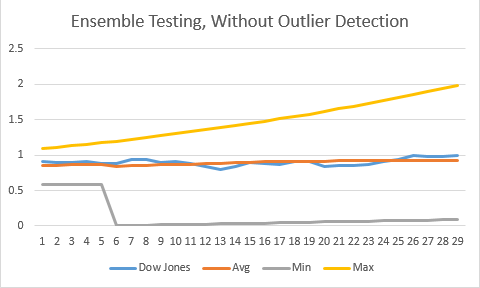
\includegraphics[width=\textwidth]{exp1/no-iflt/without-outlier-detection}
\caption{ Ensemble Testing, No Outlier Detection.}
\label{no-iflt-without-outlier}
\end{figure}

\begin{figure}[!htb]
\centering
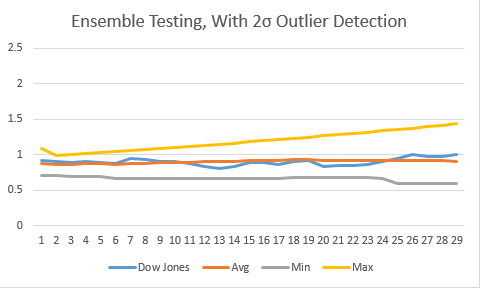
\includegraphics[width=\textwidth]{exp1/no-iflt/with-outlier-detection}
\caption{ Ensemble Testing, $2\sigma$ Outlier Detection.}
\label{no-iflt-with-outlier}
\end{figure}

\textrm{ \indent Additional work surrounding the mathematics based language includes the use of a simple automated outlier detection system. In Figures \ref{no-iflt-without-outlier} and \ref{no-iflt-with-outlier}, a comparison between no outlier prevention and an automated method is shown. Looking at the ensemble average in the first figure, it is clear to see that outliers have skewed the results. A single model at $x=11$ in the ensemble has a dramatically lower value over any other model, and thus drags the $min$ plot down. This in turn has the possibility of severely effecting the average ensemble prediction, and so needs to be addressed. In the second figure, a preventative method has been put in place.  This $2\sigma$ rule provides a range of maximum and minimum values that can models may stray from the average. It can be seen that the upper and lower bound functions surrounding the target data and average ensemble have been greatly improved by implementing this rule. This provides a somewhat statistically sound methodology to a complex problem that protects the ensemble from biased estimates. This is, however, dependent on the chosen data being normally distributed. }

\subsubsection{Discussion}

\textrm{ \indent Two common approaches to building ensembles are to average the individual models, or use the median at each time interval. Figures \ref{fig:no-iflt-avg-med} and \ref{fig:with-iflt-avg-med} show a comparison using both of these methodologies, plotted against the target data. This is shown only in the testing range, to contrast performance of each method. In using median values, an ensemble becomes very resilient to the harsh effects of outliers skewing data, but this comes at a cost. The ensemble is inherently ignoring a large number of the models it is comprised of, as it is most likely that only a few select models fall around the median for each time period. Although the average and median based ensembles perform similarly in this experiment, as the GP language becomes more complex it is likely that the median ignoring important attributes of models in the ensemble will become a more severe hindrance in accurate forecasting. }

\textrm{ \indent In the shown results, the comparison between ensembles with and without $IFLT$, $L$ and $L_{IF}$ respectively, is clear. As shown in Table \ref{no-iflt-ens-stats}, $L_{IF}$ provides favourable ensemble results regardless of the chosen fusion technique. This is likely because the use of $IFLT$ function provides each individual an alternate outlet to achieve increased volatility, and therefore closer approximate highly volatile stock data. Normally the ensemble must rely on use of cyclic trigonometric functions such as $cos$ and $sin$ to achieve this. This third resource allows individuals to create non-differentiable functions that can have sudden breaks, suiting of fitting very jagged information. }

\textrm{ \indent A major flaw to using $IFLT$ is bloat. This can behave as a safety net of sorts that allows GP to protect fitness evaluations, even if the parameters to the $IFLT$ are constant. Despite this being a possibility, the ensemble still clearly benefits from the use of this additional function. This is particularly noticeable when using averages across models as the fusion technique to build the ensemble. Consider Figures \ref{fig:no-iflt-avg-med} and \ref{fig:with-iflt-avg-med} as well as Appendix \ref{appendix-a} and \ref{appendix-b} where example GP trees for these runs are shown. It can be seen that although the GP tree is larger when $IFLT$ is included in the language, the ensemble has still proven stronger and with a marginal increase in tree size. }

\textrm{ \indent The most pronounced difference between the languages is shown when the function is in use in Figure \ref{fig:with-iflt-avg-med}. The use of average versus median ensemble fusion techniques perform nearly identically without the use of $IFLT$, which can likely be attributed to the average and median being so closely related when the language doesn't allow non-differentiable functions. This contrasts with using the additional function greatly. The strongest sign of differing features between average and median fusion techniques for $L_{IF}$ is when there is a sudden, positive directional change in the ensemble. This takes place when using average fusion. This is likely due to a model, or models, making use of the $IFLT$ function and creating a threshold that will change the slope of the generated function. This was prominent enough to become a distinct feature in the ensemble, and implies that the use of $IFLT$ is, on average, being picked up by GP rather than being ignored, as though it were not providing value. }

\textrm{ \indent The use of $2\sigma$ as a rule to protect against outliers in ensemble learning yields improved results in Figure \ref{no-iflt-with-outlier} when compared to no outlier detection in Figure \ref{no-iflt-without-outlier}. There are drawbacks, however, such as the assumption of data being normally distributed, or the disadvantage of ignoring all outliers without further consideration of what an individual data point may tell you about features of the data. In the assumption of normally distributed data, the rule is assuming that $95\%$ of the data exists within $2\sigma$ of the average. Should this not be the case, it is possible more or less will lie within this range. Regardless of this, the data is shown to be protected from bias results with the implementation of this outlier detection system. With very specified outlier detection techniques, resilience of a model or ensemble is able to be maximized. This follows with the logic of defining a GP language, in that problem specific modifications will improve a model. Despite this, the $2\sigma$ rule is not far from the estimation techniques of Veeramachaneni \textit{et al.} \cite{ensemble1}  In their work, a method is put in place where the minimum and maximum values will be estimated, and any model that exceeds these bounds is removed before being merged into the ensemble. The same system has been applied in this research. }

\textrm{ \indent A useful aspect of ensemble learning is the ability to analyse how GP is converging to a solution. This can be shown by averaging how the fitness of every model at every generation. Performing the same analysis on a single model would not be as informative, as GP is probabilistic in nature and you could not derive any conclusions from the performance of a single model. This avoids any bias regarding single models that are better by chance. Consider the graphs in Figure \ref{no-iflt-conv}. Standardized fitness is used to show the convergence pattern. A very clear increase over time is visible in the adjusted fitness plot. From here, this shows that the entire ensemble, on average, will have an adjusted fitness of $\approx 0.81$. This shows a steady convergence to a solution that clearly yields a strong ensemble fitness using a simplistic language. }

\textrm{ \indent Through the results in this experiment, it is clear that the additional Boolean function $IFLT$ in $L_{IF}$ yields stronger performance over $L$ for symbolic regression. The added flexibility in the language allows individual models to achieve a higher degree of volatility. Although over time the ensemble tapers off to relatively linear estimates, this can be attributed to having heteroskedasticity in residuals, resulting in a decrease in estimate accuracy as time goes on. The increase in performance associated with $IFLT$ creates a substantial addition to the simple math based language, defined in Table \ref{math-lang}. Further, the implementation of a programmatic outlier detection system creates a simple, robust way to avoid skewed ensemble estimates. As such, both of these additional features will be included in the remaining experiments. }

\subsection{Experiment 2: Statistics Language}

\subsubsection{Setup}

\textrm{ \indent With the inclusion of an outlier detection system, and the additional Boolean function $IFLT$, there is additional room to continue expanding the language to consider more advanced functions that may create increasingly accurate and robust systems for price forecasting using symbolic regression. Consider Table \ref{stats-lang}, where additional statistics based functions have been included in the language. The new functions are included in $L_{ST}$, and additional functions that will be considered further are defined in $L_{ST'}$. The defined language will be used to analyse performance of more advanced statistical functions. The alternate functions $avg$, $min$, and $max$ in $L_{ST'}$ are to be contrasted in the experiments as well.}

\begin{table}[h!]
\centering
\begin{tabular}{||c|c||}
\hline
 $L_{IF}$ & $x$, $ERC$, $+$, $-$, $\times$, $\div$, $log$, $cos$, $sin$, $IFLT$ \\
 \hline
 $L_{ST}$ & $L_{IF} \cup \{sum$, $stdev$, $skew$\} \\
\hline
$L_{ST'}$ & $L_{ST} \cup \{avg,\ min,\ max\}$ \\
\hline
\end{tabular}
\caption{Stats Language Definition}
\label{stats-lang}
\end{table}

\textrm{ \indent For all of the newly added functions in this experiment, a similar algorithm is followed, each applying a different rule. For example, $avg$ is used to calculate a moving average of the Dow Jones Industrial Average from time period $t_{-1}$ to $t_{-5}$, where $t$ is the current day being predicted. Likewise, $stdev$ is the standard deviation over the last 5 days, and so on for the remainder of all new functions. }

\textrm{ \indent Training data to testing data size ratios will be considered as well, deviating from the common 80-20 split to consider a 70-30 and 90-10 splits, for training data to testing data respectively. Results will be shown in an increasing order. First the 70-30 split will be shown, after which the 80-20 and 90-10 splits will be shown. This will outline clearly the behaviour that these additional functions introduce into the system, objective of the data split chosen for this experiment}

\subsubsection{Results: 70-30 Split}

% include some sample trees. 

\textrm{ \indent Consider the shown comparisons between the best individual models in the ensemble and an average fitness individual. In Figure \ref{70-inds-without} these individuals are shown under $L_{ST}$. It is clear that the curve reasonably well fit, but in testing performance both models flatten out substantially. The use of functions that take advantage of historical data is lessened without the use of $avg$, $min$, and $max$, and as a result the dependence on the past is not as prominent in these models. This dependence is much more visible in Figure \ref{70-inds-with}, under $L_{ST'}$. The best individual in the ensemble and the average individuals are actually identical under $L_{ST'}$, and it can be seen that this has very closely fit the curve. This creates an almost identical match with a slight delay. To see the GP trees created by the best model in the ensemble shown in Figure \ref{70-inds-without}, see Appendix \ref{appendix-c}. The best model in the ensemble shown in Figure \ref{70-inds-with} is shown in Appendix \ref{appendix-f}. Nearly all the models in this ensemble have a GP tree that only uses $avg$ and no other functions when using $L_{ST'}$. This is very interesting behaviour for symbolic regression, as rather than creating an equation representative of the target data, GP is able to discover the strong relationship between the $avg$ function and the data to be fit instead.}

% best avg compare
\begin{figure}[!htb]
\centering
\includegraphics[width=\textwidth]{exp2/70/without-funcs/best-avg-compare}
\caption{ 70-30 $L_{ST}$ Comparing Best \& Average Individuals.}
\label{70-inds-without}
\end{figure}

\begin{figure}[!htb]
\centering
\includegraphics[width=\textwidth]{exp2/70/with-funcs/best-avg-compare}
\caption{ 70-30 $L_{ST'}$ Comparing Best \& Average Individuals.}
\label{70-inds-with}
\end{figure}

\textrm{ \indent Similar to the comparison between individuals, the overpowering nature of the additional functions in $L_{ST'}$ is clearly visible in Figure \ref{70-ens-with}. Here the ensemble using both average and median fusion techniques is shown alongside the minimum and maximum plot lines, however they are all overlapping because they form the exact same curve. This ensemble resulted in 19 of 20 individuals with an identical GP tree, being $avg$ while one only had the small variation, as $(+\ avg\ stdev)$. In contrast with Figure \ref{70-ens-without}, it is clear that the ensemble has a diverse set of individual models. This behaviour has caused the ensemble to perform poorly relative to the use of the additional functions. Again, this raises interesting questions about the validity of this approach, because clearly GP quickly finds out that it is able to come to a very fit solution quickly. }

% ensemble testing
\begin{figure}[!htb]
\centering
\includegraphics[width=\textwidth]{exp2/70/without-funcs/ensemble-testing}
\caption{ 70-30 $L_{ST}$ Ensemble in testing}
\label{70-ens-without}
\end{figure}

\begin{figure}[!htb]
\centering
\includegraphics[width=\textwidth]{exp2/70/with-funcs/ensemble-testing}
\caption{ 70-30 $L_{ST'}$ Ensemble in testing}
\label{70-ens-with}
\end{figure}

\textrm{ \indent Although this ensemble performs poorly comparatively, it is clear that $L_{ST}$ promoted evolution over time. This is in opposition to $L_{ST'}$ which shows clear patterns of sporadic evolution in Figure \ref{70-stdfit-with}. Without the additional functions, $L_{ST}$ exhibits a smooth convergence and evolution, shown in Figure \ref{70-stdfit-without}. It is interesting that a sporadic convergence takes place at all, rather than a flat line. This behaviour implies a continued exploration of the search space that inevitably ends in choosing $avg$ as the best model in the entire run when GP is using $L_{ST'}$. }

% stdfit graphs
\begin{figure}[!htb]
\centering
\includegraphics[width=\textwidth]{exp2/70/without-funcs/standardized-fitness}
\caption{ 70-30 $L_{ST}$ Average Standardized Fitness of 20 Runs.}
\label{70-stdfit-without}
\end{figure}

\begin{figure}[!htb]
\centering
\includegraphics[width=\textwidth]{exp2/70/with-funcs/standardized-fitness}
\caption{70-30 $L_{ST'}$ Average Standardized Fitness of 20 Runs. }
\label{70-stdfit-with}
\end{figure}

\textrm{ \indent Note that due to the use of $avg$, $min$, and $max$ creating ensembles with nearly identical performance and GP trees, regardless of data splits, only the results for the 70-30 split will be shown for $L_{ST'}$. }

\subsubsection{Results: 80-20 Split}

\textrm{\indent As the use $L_{ST'}$ causes nearly identical performance regardless of the data split chosen, the only point of comparison is without the use of $avg$, $min$, and $max$, using $L_{ST}$. In Figure \ref{80-inds-without} the performance of the 80-20 split is shown for the best and average individuals in the ensemble. The GP tree for the best individual in Figure \ref{80-inds-without} under $L_{ST}$ can be seen in Appendix \ref{appendix-d}. The best individual under $L_{ST'}$ is shown in Appendix \ref{appendix-f}. In Figure \ref{80-ens-without} the performance of the 80-20 split is shown for the entire ensemble using $L_{ST}$. }

\textrm{ \indent Under $L_{ST}$ GP is still able to closely approximate the target data in testing but with certain exceptions. It seems in periods of abnormally high volatility, it is easier to generate solutions that flatten rather than attempt to match this spike in the data. Consider the first quarter of testing data in Figure \ref{80-ens-without}, before the significant drop. Here, the ensemble has averaged to approximate a line of best fit more so than a perfect regression. This is significantly more prominent in the average method of ensemble fusion, whereas the median method has managed to adequately capture some volatility in this period. This flatter approach to symbolic regression by use of averages still yields highly fit ensembles, and if GP is able to still match enough data points using this approach it is clear that it is not a threat to fitness of individuals. }

% Make captions on graphs more unique
\begin{figure}[!htb]
\centering
\includegraphics[width=\textwidth]{exp2/80/without-funcs/best-avg-compare}
\caption{ 80-20 $L_{ST}$ Comparing Best \& Average Individuals.}
\label{80-inds-without}
\end{figure}

\textrm{ \indent In Figure \ref{80-inds-without} interesting behaviour is seen in both the best individual in the ensemble, as well as one of average fitness. Notice that this uses language $L_{ST}$, and still creates behaviour similar to what is expected from the $avg$ function. The best individual in this example clearly shows a very tight bound to the target data, and this is because it has discovered the use of $avg$ implicitly, through use of alternate functions in the language. Specifically, the GP tree for that model is $(*\ C[0.2044]\ sum)$. Recall that $sum$ is a summation of the target data over the last 5 days, and so by multiplying the sum by a constant $0.2044$, it is really taking the average. The average fitness individual also behaves similarly, but with a looser bound surrounding the target data both in training and testing. This model's GP tree is $(cos\ (sin\ (cos\ sum)))$ and although it is not calculating the average implicitly, it has still discovered the tight relationship that $sum$ has to the target data. }

\begin{figure}[!htb]
\centering
\includegraphics[width=\textwidth]{exp2/80/without-funcs/ensemble-testing}
\caption{ 80-20 $L_{ST}$ Ensemble in Testing.}
\label{80-ens-without}
\end{figure}

\subsubsection{Results: 90-10 Split}

\textrm{ \indent Finally, the results of the 90-10 split are shown. In Figure \ref{90-inds-without} a comparison is shown between the best and average individuals from the ensemble. Because the 90-10 split has the shortest testing range, it can be expected to fit the target data closer than any of the other data splits. This does, however, draw awareness to the potential of overfitting data and achieving less meaningful results. }

\textrm{ \indent Much like the 80-20 split, as well as the 70-30 split, there exists a diverse set of individual models in the ensemble when the language $L_{ST}$ is used. The average individual shown in Figure \ref{90-inds-without} has many completely flat portions, while the most fit actually seems as though it is using the $avg$ function, given how closely it is approximating the curve and the results shown in Figure \ref{70-inds-with}. This cannot be the case, however, as this function is not included in $L_{ST}$. To see the GP tree that creates this behaviour, see Appendix \ref{appendix-e}. For the GP tree under $L_{ST'}$ see Appendix \ref{appendix-f}. In this case, the best individual in the ensemble for both the 80-20 split as well as the 90-10 split, shown in Figures \ref{80-inds-without} and \ref{90-inds-without} respectively, has discovered the use of $avg$ by means of alternate functions. Specifically both models have the GP tree $(*\ C[0.2049]\ sum)$, a very close approximation of $avg$, as it has discovered that $(\approx \frac{1}{5}\cdot sum)$ yields highly fit individuals. }

% Make captions on graphs more unique
\begin{figure}[!htb]
\centering
\includegraphics[width=\textwidth]{exp2/90/without-funcs/best-avg-compare}
\caption{ 90-10 $L_{ST}$ Comparing Best \& Average Individuals.}
\label{90-inds-without}
\end{figure}

\textrm{ \indent Most models in the ensemble do not take advantage of the indirect usage of the $avg$ function. This allows the high fitness of this function to be applied without ridding the ensemble of diversity of individuals. The ensemble performance in testing data for the 90-10 split is shown in Figure \ref{90-ens-without}. As mentioned previously, the 90-10 split has the shortest testing range and as such can be expected to be the closest approximation of the target data. This is particularly true when you contrast with Figure \ref{70-ens-without}, where the testing range starts with high data and includes a steep drop, whereas Figure \ref{90-ens-without} is increasing at a relatively consistent rate throughout.}

\begin{figure}[!htb]
\centering
\includegraphics[width=\textwidth]{exp2/90/without-funcs/ensemble-testing}
\caption{ 90-10 $L_{ST}$ Ensemble in Testing.}
\label{90-ens-without}
\end{figure}

\textrm{ \indent Consider Table \ref{data-split-results} where the numeric results of each of the mentioned experiments is shown. This compares the use of the additional functions $avg$, $min$, and $max$ in $L_{ST'}$ to $L_{ST}$, as well as the given data split and outliers removed from each ensemble. Fitness is shown in the first two rows for each data split both with and without the use of the mentioned additional functions. Similarly, the number of outlier data points removed from the ensemble is given for each data split for $L_{ST}$ and $L_{ST'}$. Note that standardized fitness is only given for the average fusion technique for creating the ensemble, despite graphically showing the median technique as well. This is due to their similar performance and the mentioned behaviour inherent to the average technique over median.}

\begin{table}[!ht]
\centering
\begin{tabular}{||c|c|c|c||}
\hline
 & \textbf{70-30} & \textbf{80-20} & \textbf{90-10} \\
 \hline
 \textbf{$L_{ST'}$ Fitness} & 0.088749 & 0.074097 & 0.026279 \\
 \hline
 \textbf{$L_{ST}$ Fitness} & 1.395065 & 0.246555 & 0.073232 \\
 \hline
 \textbf{$L_{ST'}$ Outliers Removed} & 466 & 310 & 111 \\
 \hline
 \textbf{$L_{ST}$ Outliers Removed} & 384 & 253 & 18 \\
 \hline
\end{tabular}
\caption{Stats Language Performance}
\label{data-split-results}
\end{table}

\textrm{ \indent In the results table a clear superiority is shown by the 90-10 split. However, it is important to consider that purely comparing the standardized fitness of each data split is a slightly skewed methodology. This is because any data split with a testing range larger than another data split will inherently also include the sum of errors over the same set of data points as the smaller data split, as well as the extended range. For example, the 80-20 split uses the last 20\% of the data as testing, and the 90-10 split uses the last 10\%, but of course the 80-20 split will include the last 10\% as well. As such, the comparison needs to be drawn lightly. It is worth noting in this case that despite the drawback to this method of comparison, a large distinction is made by the 90-10 split. The difference between the 70-30 and 80-20 split is not nearly as large as the difference between the 80-20 and the 90-10, despite the same relative gap in data size. This persists regardless of the chosen language variant. It is also worth noticing that there exist very few outliers in the 90-10 split using $L_{ST}$. This is suggestive of the model's confidence improving in this data split. This points toward less exploration of the problem search space as comparatively few individuals ever exceed the $2\sigma$ bound surrounding the ensemble average. }

\subsubsection{Discussion}
% discuss the (* sum C[0.204]) trees seen in 80-20 and 90-10 split.

\textrm{\indent In all cases in Table \ref{data-split-results} the use of the additional functions $avg$, $min$, and $max$ in language $L_{ST'}$ yield higher standardized fitness in testing. This raises interesting questions regarding the use of $avg$ as a rule of thumb for price forecasting. In this sense, the use of $L_{ST'}$ has approached the idea of rule-based GP over symbolic regression. The matter of whether or not this creates an overfit ensemble is also interesting. Despite not finding patterns and features of the target data, GP has found that estimating through use of the average over the last week is a good enough rule when it is an option. When the $avg$ function is not present in the language, such as with $L_{ST}$, GP still manages to find the use of averages as a general rule but without sacrificing diversity in the ensemble as a result, as seen in the results shown. Because of this, a close analysis between these methods should be done. It is normally expected that the models with the lowest standardized fitness should always perform the best, but it should be noted that forecasting 30\% of the target data versus 10\% are two very different problems, and as such having just a lower standardized fitness is only partially indicative of a true increase in performance. When $L_{ST'}$ is the chosen language, the use of $avg$ is clearly the first choice for GP, but without using these additional functions the models have been shown to still discover the rule of $avg$ using the GP tree $(*\ C[0.2049]\ sum)$, which in standard mathematical notation is $0.2049\times sum = \frac{sum}{5}$. }

\textrm{ \indent Given that the ensembles yield a substantially higher standardized fitness for the 90-10 split, what must be considered is why. The 90-10 data split provides the largest amount of training data for GP to learn from, but consequently also has the smallest testing set. This is inherent to the problem in comparing data split techniques in this way. The 70-30 data split will always have the poorest standardized fitness because it includes the testing ranges from both the 80-20 split and the 90-10 split. Because of this, the differences between them must be considered. In Table \ref{data-split-results} the marginal difference between the 90-10 data-split is stronger than the opposing techniques. The marginal change in size between 70-30 to 80-20 is the same from 80-20 to 90-10. This implies that the smaller testing data set size is not the only reason for an improvement in fitness. }

\textrm{ \indent When using $avg$, the ensemble is completely skewed as most, if not all, individuals have a heavy dependence on this function. This results in models that do fit the target data in testing and yield the best standardized fitness scores shown, but GP is not evolving in the way it is generally intended to. If the evolution patterns shown in Figures \ref{70-stdfit-with} and \ref{70-stdfit-without} are to be considered, it is clear that without these functions a steady and consistent convergence takes place. This indicates that the ensemble is picking up on features and attributes of the target data that can be used in forecasting. This is not the case when using the additional functions, with any data split. GP does continue exploring the search space but always settles on using $avg$. }

\textrm{ \indent Considering this increase in performance comes at the cost of hiding all performance indicators from any other functions in the language, the language variant $L_{ST'}$ will again be considered in the final experiment along with the added financial functions to properly analyse the effect this may have. Throughout the duration of these experiments, all three of the mentioned additional functions were included in the language variations. It is notable that when only $min$ and $max$ were included, GP behaves similarly only favouring $max$ instead of $avg$. This behaviour also applies when only $min$ is included as the additional function to the language. It is likely that $min$ is outperformed slightly by $max$ because, in the long run, the target data chosen is increasing. If the target data were decreasing over time, it is expected the inverse effect would be displayed. The shown behaviour is interesting in that GP will discover shortcuts of this nature even if they are not explicitly provided in the language, but analysis of additional financial functions in the final experiment must be considered both with and without these functions due to the discussed nature of the $avg$ function on the ensemble. }

\subsection{Experiment 3: Financial Language}

\subsubsection{Setup}

\textrm{ \indent This experiment will consider the use of advanced functions that make use of historical data features associated with the Dow Jones Industrial Average being forecast. These functions are $open$, $high$, $low$, and $vol$, representing the open price, high, low, and volume traded on the index 5 days prior. Note that $close$ is not included as this is the feature being predicted. This language variant is defined as $L_{FI}$ in Table \ref{finance-lang}. }

\begin{table}[h!]
\centering
\begin{tabular}{||c|c||}
\hline
$L_{ST}$ & $x$, $ERC$, $+$, $-$, $\times$, $\div$, $log$, $cos$, $sin$, $IFLT$, $sum$, $stdev$, $skew$ \\
\hline
$L_{FI}$ & $L_{ST} \cup open$, $high$, $low$, $vol$ \\
\hline
$L_{FI'}$ & $L_{FI} \cup \{ avg$, $min$, $max\}$ \\
\hline
\end{tabular}
\caption{Finance Language Definition}
\label{finance-lang}
\end{table}

\textrm{ \indent All findings from previous experiments have been included into this experiment, allowing for the use of $IFLT$, as well as using a 90-10 data split for improved performance. The additional functions $avg$, $min$, and $max$ from the previous experiment will again be considered in $L_{FI'}$ and analysed in conjunction with the newly added functions in this experiment. This is to gauge how the overpowering nature of $avg$ may perform with more advanced functions such as those newly defined in $L_{FI}$. These functions draw strong relationships to the $close$ price that is being estimated, and as a result it is expected that the most fit individuals in these experiments will rely heavily on them. }

\subsubsection{Results}

\textrm{ \indent Consider Figures \ref{exp3-inds-without} and \ref{exp3-inds-with}. These graphs plot nearly the same behaviour, however Figure \ref{exp3-inds-with} is using the language variant $L_{FI'}$, while Figure \ref{exp3-inds-without} is $L_{FI}$. Notice that in both cases, an average fit individual is plotted as well as the most fit individual model from the entire ensemble. This shows clearly that the financial functions create behaviour very similar to what was described in regards to $avg$ in the prior experiment. }

\begin{figure}[!htb]
\centering
\includegraphics[width=\textwidth]{exp3/without/best-avg-compare}
\caption{ $L_{FI}$ Comparing Best \& Average Individuals.}
\label{exp3-inds-without}
\end{figure}

\textrm{\indent The majority of models in Figure \ref{exp3-inds-with} under $L_{FI'}$ still result in the GP tree of just $avg$. In Figure \ref{exp3-inds-without}, similar behaviour is shown only with regards to the $high$ function. Many of the individual models use only this function, or a small variation with few other functions included. This creates a very similar pattern, closely following the target data with a 5 day lag.  }

\begin{figure}[!htb]
\centering
\includegraphics[width=\textwidth]{exp3/with/best-avg-compare}
\caption{ $L_{FI'}$ Comparing Best \& Average Individuals.}
\label{exp3-inds-with}
\end{figure}

\textrm{ \indent A closer distinction between the behaviours of the newly added financial functions and the functions $L_{FI'}$ can be seen in the testing of the ensemble. This is shown in Figures \ref{exp3-ens-without} and \ref{exp3-ens-with}. Because the experimental functions have a tendency to rely on $avg$, the ensemble forms a smooth curve that generally behaves as a line of best fit to the target data. This is not the case when these functions are excluded from the language in $L_{FI}$, as the $high$ function uses a single days value, and so even when averaged over the ensemble will still result in significantly more volatile data than what is seen in using the additional functions. This can prove to prove to create an upper bound to the target data at a minor delay. It is interesting to consider the data having shifted the ensemble back 5 days, simply to observe the close relationship it exhibits to the target data. This is shown in Figure \ref{exp3-lag-shown}. It is interesting to see how closely the target data is able to be fit by the ensemble in this case. Note that the majority of functions in this ensemble are some variant of $high$, so in cases where there are gaps between the target data and the ensemble, it is almost always creating an upper bound. This is informative of how to properly perceive results generated by the language $L_{FI}$.  }

\begin{figure}[!htb]
\centering
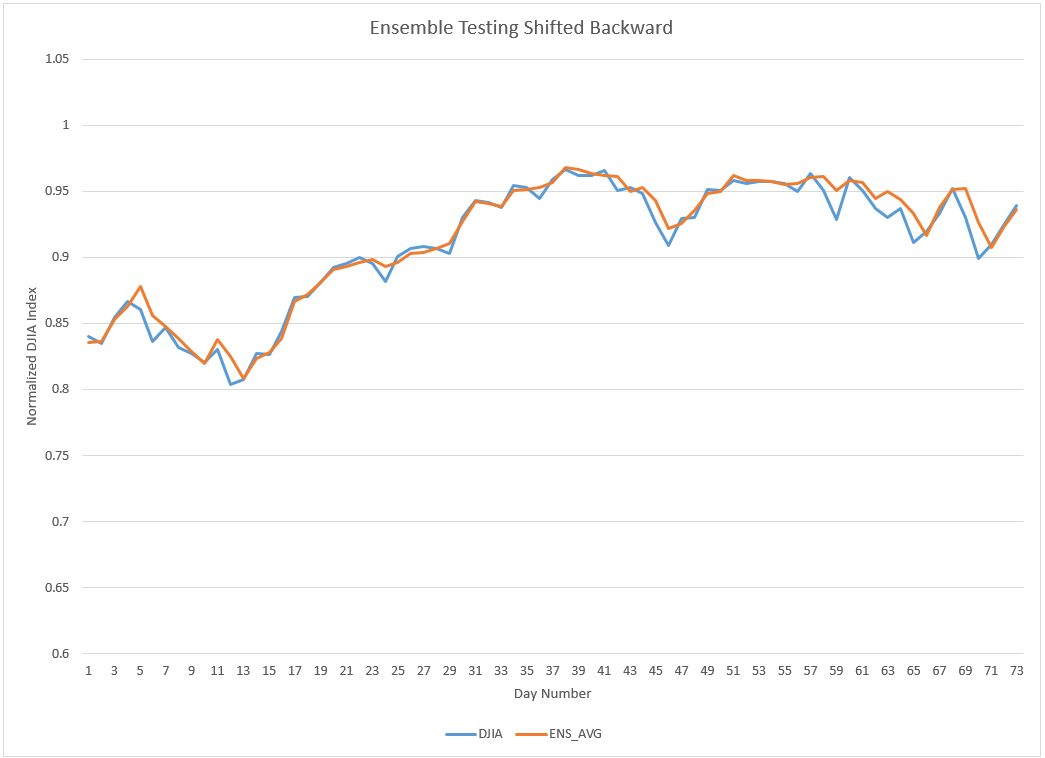
\includegraphics[width=\textwidth]{exp3/without/ensemble-testing-shifted}
\caption{ $L_{FI}$ Ensemble Shifted 5 Days in Testing.}
\label{exp3-lag-shown}
\end{figure}

\begin{figure}[!htb]
\centering
\includegraphics[width=\textwidth]{exp3/without/ensemble-testing}
\caption{ $L_{FI}$ Ensemble in Testing.}
\label{exp3-ens-without}
\end{figure}

\begin{figure}[!htb]
\centering
\includegraphics[width=\textwidth]{exp3/with/ensemble-testing}
\caption{ $L_{FI'}$ Ensemble in Testing.}
\label{exp3-ens-with}
\end{figure}

\textrm{ \indent Consider the results of this experiment in Table \ref{exp3-results}. Here the performance of the financial language is shown with and without the use of the additional functions $avg$, $min$, and $max$. Similar to what is shown in Experiment 2, the use of these functions does yield a stronger fitness but is essentially creating a rule to always rely on the average over the previous five days.   }

\begin{table}[!ht]
\centering
\begin{tabular}{||c|c|c||}
\hline
 & \textbf{Ensemble Std. Fit} & \textbf{Outliers Removed} \\
\hline
$L_{FI}$ & 0.057844 & 128 \\
\hline
$L_{FI'}$ & 0.026279 & 0 \\
\hline
\end{tabular}
\caption{Finance Language Performance}
\label{exp3-results}
\end{table}

\subsubsection{Discussion}

\textrm{ \indent In this experiment, the added financial functions performed well without relying on the $avg$ function, but only when using $L_{FI'}$. It can be seen that when using $L_{FI}$, by relying mostly on $high$ GP is able to capture a level of volatility akin to the target data. This boasts well for the inclusion of these functions in the language. By relying on the $avg$ function, a better fitness is found but this nullifies the use of any additional functions introduced in this experiment. Additionally, this creates a very smooth curve that behaves similarly to a line of best fit. As price data for the Dow Jones Industrial Average is very volatile, much like many other indexes, the ability to capture this volatility is important for short term forecasting. Long term growth, however, is heteroskedastic when capturing this volatility. This means that as time goes on, mean squared error is increasing. When using the $avg$ function this is visibly not the case, as shown in Figure \ref{exp3-ens-with}, where the curve trends follow more closely along the generic growth pattern shown. }

\textrm{ \indent The use of the various additional functions in $L_{FI'}$ becomes one of weighing the pros and cons for each. Although the $avg$ function yields strong fitness scores, it fails to capture short term variability in the index being estimated. Without these, the financial functions in $L_{FI}$ do a good job of maintaining some diversity of models in the ensemble while still capturing volatility in the short term. This is shown particularly well when comparing Figure \ref{exp3-ens-without} to Figure \ref{exp3-ens-with}. Note the substantial increase in volatility shown when using $L_{FI}$. At this point, the decision to include certain functions in the language is dependent on the forecaster's goal. Should short-term trading be of interest, perhaps a smoother curve generated by $avg$ is less appealing, as this is indicative of growth patterns more than it is of day-to-day fluctuations. The added financial functions do an excellent job of measuring these smaller changes, and so may be best utilized under this pretense. }

\newpage 

\section{Conclusion}

% General experiment 1
\textrm{ \indent The additions to the GP language throughout these experiments show a clear improvement in forecasting ability for the system. However, more advanced functions have been shown to produce unexpected behaviour. Through use of the purely mathematical language $L$ discussed in Experiment 1, a strong GP ensemble is created that performs symbolic regression moderately well. The added function $IFLT$ in $L_{IF}$ is a clear benefit to the system, eliminating the harsh cyclic effects commonly attributed to functions such as $cos$ and $sin$ while still being able to capture volatility seen in the target data. In doing this, a very general direction of growth is created but errors quickly increase in the testing phase. This is due to the fact that in a purely mathematical language, there is no dependence on the data analogous to the more advanced statistical and financial languages. This makes GP commonly continue growth in the direction it was heading at the end of the training period. This is the most common attribute among the results of the first experiment. If the testing period is such that the data does not include many sudden troughs or peaks, a line of best fit is created that reasonably fits the target data. }

% Outlier detection system
\textrm{ \indent The use of the automated outlier detection system discussed in Experiment 1 is also an important asset to the remainder of experiments. Although explicit comparisons are not shown, there are multiple cases in Experiment 2 and Experiment 3 where minimum and maximum plot lines are sporadic, likely as a result of removing outlier data points from the series. Given the severity of outliers on an averages fusion technique for ensemble building, the use of a simple $2\sigma$ rule is a quick fix for what is such an adverse effect on performance. The use of a similar technique by Veeramachaneni \textit{et al.} \cite{ensemble1} shows promise for this approach creating a general upper and lower bound with which expected data may exist. Interestingly, outliers removed increases as the language became more advanced, with the exception of the behaviour seen with the $avg$ function. This can be seen when comparing Table \ref{no-iflt-ens-stats} to Tables \ref{data-split-results} and \ref{exp3-results}. When using the $avg$ function in the final experiment there were 0 outliers removed while in all other cases the number of outliers removed, when considering only the same data split of 90-10, is generally larger. Due to the shown behaviour of the $avg$ function, it is expected there be fewer outliers as nearly all models in the ensemble resulted in the same GP trees when $avg$ was included in the language. }

% Data split
\textrm{ \indent When considering the results of Experiment 2 it is important to consider the differences involved in comparing the standardized fitness across multiple data split methods. It is clear from Table \ref{data-split-results} that the 90-10 training to testing data split yields the highest performance. This is to be taken lightly, as the larger data splits will inherently contain the data in the smaller data splits, and as such will always result in a higher, and thus poorer, standardized fitness. Due to this, a substantially lower standardized fitness is only partially suggestive of an improvement to the system. Consider the right most column of Table \ref{data-split-results}, where it is clear that the 90-10 split has performed the best. Here, the marginal difference between the 90-10 split and the 80-20 split is substantially higher than between the 70-30 and the 80-20 in all categories. This implies that the increase in performance can be accredited to more than a shorter testing period. There are substantially fewer outliers in each case, and each with the best fitness scores in the experiment. Despite being able to see that the 90-10 data split is the best overall, a better approach for future work would be to consider cross validation. This would involve dividing the data into three categories, training, validation and testing, rather than two used. A constant testing size would be chosen, and the ratio between training and validation would be experimented on. This would allow an equal comparison of standardized fitness as the testing period would always be the same length. This would then provide an outlet to analyse more closely which data split truly provides the best performance without creating an overfit ensemble, and without the difficulty in comparison discussed in this experiment. }

% use of Avg, min and max in the language.
\textrm{ \indent In both Experiment 2 and Experiment 3, the use of an alternative language was discussed. This language variant would take the improved language from the previous experiment, along with any newly added functions, and consider their use in conjunction with $avg$, $min$, and $max$. This is shown in $L_{ST'}$ and $L_{FI'}$, compared to $L_{ST}$ and $L_{FI}$ respectively. In both cases, the inclusion of the additional functions always yielded a skewed ensemble that showed preference to the $avg$ function. Although this is not performing the expected behaviour of symbolic regression, the discovery made is that the $avg$ function ties very closely to the target data. This effect is strong enough that GP uses this as a shortcut to very quickly achieve fit models. This is analogous to rule based genetic programming in that rather than focusing on fitting the curve, this general rule can be applied to approximate the target data in the future. }

\textrm{ \indent As shown in Figures \ref{70-stdfit-without} and \ref{70-stdfit-with} the convergence behaviours in the ensemble strongly imply that the use of the additional functions in $L_{ST'}$ and $L_{FI'}$ attempt to explore the search space, but always result in $avg$ as the most fit individual for that run. Also noteworthy is that when $avg$ was excluded from the language but $max$ or $min$ were included, GP still exhibits a tendency to prefer them over any other functions in the language. This is likely due to $max$ and $min$ not straying far from the average over the last week in most cases. The relationship between $avg$ must then be the closest to the target data, but $max$ and $min$ still yield highly fit individuals while overriding any diversity in the ensemble. This close relationship to the target data can be well used for long-term forecasting. Although the $avg$ function does not closely approximate highly volatile periods of time, long-term growth can be easily forecast with this method given the more conservative nature of averages in the system.  }

%finance functions
\textrm{ \indent Similar to the affect seen by using $avg$, the financial functions generally yield very small GP trees due to their close relationship to the target data. In Experiment 3 when comparing $L_{FI}$ with the additional functions in $L_{FI'}$, very few individuals in either ensemble had large trees. When the additional functions were included in $L_{FI'}$ the most fit individual in the ensemble did not explicitly use $avg$. The GP tree for this model is shown in Appendix \ref{appendix-h}. Here it is seen that a few functions are used, but this model will actually behave identically to $avg$. This is because $low$ is always going to be less than $(sin\ sum)$, and so the else case of the $IFLT$ function is always used. This is an interesting, minor example of bloat. Although bloat was discussed previously, it did not come to be a problem in any of the experiments. In this case, GP protects fitness despite always being false in the $IFLT$ function, always returning $avg$.  }

\textrm{ \indent Another feature that is interesting to note is that the standardized fitness of the ensemble that makes use of these additional functions is actually identical to the standardized fitness shown in Table \ref{data-split-results} for the 90-10 split. The newly added financial functions in $L_{FI}$ have no impact on the language when $avg$, $min$, and $max$ are included in $L_{FI'}$, although the performance without the additional functions remains higher than the 90-10 split shown in Table \ref{data-split-results} without these functions. The financial functions, then, have still yielded an improvement to the language when analysed without the impact of the overpowering statistical functions discussed throughout Experiment 2 and Experiment 3. }

\textrm{ \indent Across the experiments, the most outstanding results were shown with the most advanced languages $L_{FI}$ and $L_{FI'}$. This used a 90-10 data split, as well as all functions from earlier experiments. Also included was the discussed automated outlier detection system. This creates a cumulative attempt using the best found results to build a truly robust GP system based on symbolic regression for financial forecasting. The use of the added functions $avg$, $min$, and $max$ in $L_{FI'}$ yielded the strongest results throughout all experiments, even having exactly 0 outliers removed in the final iteration. The use of financial and statistical functions over simpler mathematical functions has been shown to provide substantially stronger GP models, and through use of ensemble learning approximate forecasts are more safely predicted by keeping track of the minimum, maximum, standard deviation, median, and average of the ensemble. }

\textrm{ \indent An industry application of this work could provide the end user with a full interface, presenting language variations as well as parametric options to the user based on their desired method of forecasting. This potential improvements point towards some of the work done by Veeramachaneni \textit{et al.} \cite{ensemble2}. In his research, ensemble learning based GP is applied in a dynamic, cloud based system that uses a live data stream and an outlier detection method similar to the proposed methodology in Experiment 1. For short-term forecasting, and potentially day trading, GP with ensemble learning, a language variant like $L_{FI}$, and a median based ensemble fusion technique has been shown to yield strong results. This is because of the increased volatility associated with the median ensemble and the language without functions like $avg$. For long-term forecasting, one could instead use average ensemble fusion techniques with the additional functions $avg$, $min$, and $max$ due to it's reduction in variance of mean squared errors and stability in the long run. Additional future work could explore array-based GP functions that are capable of applying operators to a series of data points rather than a single input. This is analogous to some of the functions like $avg$ that compute a value over a range of data, but an interesting application could allow the discovery of dynamic functions applied to data ranges by GP.  }

\newpage 

\begin{appendices}
\appendix
\section{$L$ Best Model from Ensemble}
\label{appendix-a}
\setstretch{1.0}
\begin{lstlisting}
(* C[0.477288858984907] (log (log (+ (/ (/ (log (/ (log (+ (* (/ x x) (/ (* C[0.07099347687193136] (* x C[0.1688777841243665])) (/ C[0.7133551833503038] (log (* (+ x C[0.7347957341403779]) (cos x)))))) x)) C[0.477288858984907])) (* C[0.477288858984907] (/ (* C[0.07099347687193136] x) (/ x x)))) (* C[0.477288858984907] (* C[0.07099347687193136] x))) (+ (/ (* C[0.07099347687193136] x) (/ (/ (/ (log (+ (/ (log (+ C[0.5578493843039484] (* C[0.07099347687193136] x))) C[0.2525903380189627]) x)) (* (* C[0.477288858984907] (/ (* C[0.07099347687193136] x) (/ (/ (/ x (log x)) (* C[0.07099347687193136] x)) C[0.2525903380189627]))) (/ (* C[0.07099347687193136] (* (* x C[0.1688777841243665]) C[0.7701707675343847])) (/ x x)))) (* C[0.477288858984907] (/ (* C[0.07099347687193136] x) (/ (/ (log (+ C[0.5578493843039484] x)) (* C[0.07099347687193136] x)) C[0.2525903380189627])))) (* C[0.477288858984907] (log (log (* C[0.477288858984907] (/ (* C[0.07099347687193136] x) (/ (/ (/ x (log x)) (* C[0.07099347687193136] (+ C[0.5578493843039484] x))) C[0.2525903380189627])))))))) x)))))
\end{lstlisting}

\section{$L_{IF}$ Best Model from Ensemble}
\label{appendix-b}
\setstretch{1.0}
\begin{lstlisting}
(sin (log (* (log (cos (sin (log (* (log (* (IFLT (log x) (* (* x C[0.014937200025926467]) (IFLT (log (sin (cos C[0.08928159658424939]))) (/ (log (log x)) (* x x)) x (log C[0.7747255157329026]))) (cos (log (log x))) (+ (IFLT x (log (log x)) x C[0.6503002101970727]) (/ C[0.8461758134385032] (* (cos (log C[0.8344959091126747])) (log (* C[0.496538161680536] x)))))) (* (log x) (log C[0.7747255157329026])))) (* (log x) (log C[0.7747255157329026]))))))) (* (log (IFLT (IFLT (cos (log C[0.7747255157329026])) (* (log x) C[0.37209043557694077]) (IFLT C[0.7747255157329026] (/ x (- (- x x) (* (IFLT (+ x (* C[0.1864861319928771] x)) C[0.34825105946220825] (sin (IFLT C[0.8065547190739079] C[0.7570846100070036] x C[0.4662835580009185])) (/ C[0.78649020032555] (log x))) (* (cos C[0.536790979023098]) (* x x))))) (* (cos (* C[0.496538161680536] x)) (log (log x))) (IFLT x (log (log x)) (cos (+ (* (cos (cos (* C[0.496538161680536] x))) (log (log x))) (* (cos (* (log x) (log C[0.7747255157329026]))) (log (log x))))) (* (/ C[0.78649020032555] (log x)) (/ C[0.8461758134385032] (* (cos C[0.7971251702196291]) (* (log x) (log C[0.7747255157329026]))))))) (+ (IFLT x (log (* C[0.496538161680536] x)) (log C[0.7747255157329026]) C[0.6503002101970727]) (/ C[0.8461758134385032] (* (log (log (log C[0.8344959091126747]))) (* (log x) (log C[0.7747255157329026])))))) (sin C[0.04645635786535329]) x (IFLT (* (cos C[0.08928159658424939]) (* (log x) (/ x (- (- x x) (* (IFLT (cos (cos x)) C[0.34825105946220825] (sin (IFLT C[0.8065547190739079] C[0.7570846100070036] x C[0.4662835580009185])) (/ C[0.78649020032555] (log x))) (* (cos C[0.536790979023098]) (* x x))))))) x (+ (* C[0.1864861319928771] x) x) (log C[0.21979534452930316])))) (log (log (log C[0.8344959091126747])))))))
\end{lstlisting}

\section{$L_{ST}$ 70-30 Best Model from Ensemble}
\label{appendix-c}
\setstretch{1.0}
\begin{lstlisting}
(cos (IFLT stdev (cos (log x)) (IFLT (log (sin (cos (cos (log x))))) (IFLT (cos (cos (log C[0.8551785929447195]))) C[0.01892335652084054] C[0.9117344446374672] (sin (+ (cos (log C[0.8551785929447195])) (log x)))) (sin (sin C[0.37196542216076256])) (sin (IFLT (IFLT (cos (cos (log x))) (IFLT (cos C[0.3856672776693868]) C[0.01892335652084054] C[0.9117344446374672] (sin (cos (cos (sin (cos C[0.37196542216076256])))))) C[0.9117344446374672] (sin (IFLT (cos (sin (cos C[0.37196542216076256]))) C[0.01892335652084054] C[0.9117344446374672] (IFLT (cos (cos (log x))) C[0.9117344446374672] (cos (log (cos (log x)))) (log x))))) (cos (log x)) (sin (cos (cos (log x)))) (cos (cos (log x)))))) (cos (sin (sin (sin (sin (sin (log x)))))))))
\end{lstlisting}

\section{$L_{ST}$ 80-20 Best Model from Ensemble}
\label{appendix-d}
\setstretch{1.0}
\begin{lstlisting}
(* C[0.2043872969831534] sum)
\end{lstlisting}

\section{$L_{ST}$ 90-10 Best Model from Ensemble}
\label{appendix-e}
\setstretch{1.0}
\begin{lstlisting}
(* sum C[0.2041923607950923])
\end{lstlisting}

\section{$L_{ST'}$ Best Model from Ensemble (All Data Splits)}
\label{appendix-f}
\setstretch{1.0}
\begin{lstlisting}
avg
\end{lstlisting}

\section{$L_{FI}$ Best Model from Ensemble}
\label{appendix-g}
\setstretch{1.0}
\begin{lstlisting}
high
\end{lstlisting}

\section{$L_{FI'}$ Best Model from Ensemble}
\label{appendix-h}
\setstretch{1.0}
\begin{lstlisting}
(IFLT low (sin sum) (- avg min) avg)
\end{lstlisting}

\end{appendices}

\newpage

\addcontentsline{toc}{section}{Bibliography}
\bibliographystyle{abbrv}
\bibliography{thesis}

\end{document}